\documentclass[UTF8]{ctexart}
\usepackage{amsmath}
\usepackage{amssymb}
\usepackage{graphicx}
\usepackage{geometry}
\usepackage{ctex}
\usepackage{amsmath}
\usepackage{amssymb}
\usepackage{xcolor}
\usepackage{geometry}
\usepackage{listings}
\usepackage{geometry}
\usepackage{marginnote}

\geometry{a4paper, margin=1in}

% Style for code blocks
\definecolor{codegreen}{rgb}{0,0.6,0}
\definecolor{codegray}{rgb}{0.5,0.5,0.5}
\definecolor{codepurple}{rgb}{0.58,0,0.82}
\definecolor{backcolour}{rgb}{0.95,0.95,0.95}

\lstdefinestyle{mystyle}{
    backgroundcolor=\color{backcolour},   
    commentstyle=\color{codegreen},
    keywordstyle=\color{magenta},
    numberstyle=\tiny\color{codegray},
    stringstyle=\color{codepurple},
    basicstyle=\ttfamily\footnotesize,
    breakatwhitespace=false,         
    breaklines=true,                 
    captionpos=b,                    
    keepspaces=true,                 
    numbers=left,                    
    numbersep=5pt,                  
    showspaces=false,                
    showstringspaces=false,
    showtabs=false,                  
    tabsize=2
}
\lstset{style=mystyle}
\geometry{a4paper, margin=1in}

\title{QTA2025暑期求职笔试训练营-week2}
\author{}
\date{}

\begin{document}

\maketitle

\section*{笔试题目}

\subsection*{1. 随机数}
小U有一个质地不均匀的硬币, 已知这枚硬币正面朝上的概率$p$不是0或0.5, 但不知道确切的概率, 可以只用这枚硬币帮小U生成100个0-15之间均匀分布的随机整数吗? 小U是个追求严谨的小朋友, 如果可以, 需要聪明的你证明这种策略下生成的随机数的分布严格服从上述要求; 如果不可以, 也请给出证明。

这个问题的核心在于如何利用有篇的随机源来构建概率均等的随机数,我们考虑如下策略,将硬币连续抛掷两次 :
\begin{itemize}
    \item 如果结果是 正-反 (HT),我们就将其记为 0。

    \item 如果结果是 反-正 (TH),我们就将其记为 1。
    
    \item 如果结果是 正-正 (HH) 或 反-反 (TT),我们就舍弃这次结果,重新抛掷两次。    
    
\end{itemize}

\textbf{第一步:验证该策略确实可以生成我们要求的随机数}

设硬币正面朝上的概率为 $p$,反面朝上的概率为 $1-p$(其中 $p \neq 0, 0.5, 1$)。

计算各种情况的概率:
\begin{align}
P(HT) &= p \cdot (1-p) \\
P(TH) &= (1-p) \cdot p = p \cdot (1-p) \\
P(HH) &= p^2 \\
P(TT) &= (1-p)^2
\end{align}

注意到$P(HT) = P(TH) = p(1-p)$

在条件概率下:
\begin{align}
P(\text{输出0} | \text{不拒绝}) &= \frac{P(HT)}{P(HT) + P(TH)} =
\frac{p(1-p)}{2p(1-p)} = \frac{1}{2} \\
P(\text{输出1} | \text{不拒绝}) &= \frac{P(TH)}{P(HT) + P(TH)} =
\frac{p(1-p)}{2p(1-p)} = \frac{1}{2}
\end{align}

因此,每次生成的随机数都是公平的,即 $P(\text{输出0}) = P(\text{输出1}) =
\frac{1}{2}$。

\textbf{第二步:生成0-15的均匀分布}

考虑到是生成16个数,我们可以二进制来处理,具体来说:
\begin{enumerate}
    \item 使用上述方法生成4个概率均等的随机数 $b_3b_2b_1b_0$
    \item 将这上面的随机数转换为整数:$n = 8b_3 + 4b_2 + 2b_1 + b_0$
    \item 由于 $n \in \{0,1,2,\ldots,15\}$,直接输出 $n$
\end{enumerate}


由于每次生成的单个随机数都是独立且公平的($P(b_i = 0) = P(b_i = 1) = \frac{1}{2}$),所以:

$$P(n = k) = P(b_3b_2b_1b_0 \text{的二进制表示为} k) = \left(\frac{1}{2}\right)^4 =
\frac{1}{16}$$

对于所有 $k \in \{0,1,2,\ldots,15\}$ 都成立。

\textbf{第三步:生成100个随机数:}

重复上述过程100次,每次生成一个0-15之间的随机整数。由于每次生成都是独立的,且每个整
数的概率都是 $\frac{1}{16}$,所以生成的100个数严格服从0-15的均匀分布。

\subsection*{2. 剪纸转圈圈}
\subsubsection*{(1)}
小U在做剪纸小游戏, 他先剪了一大一小两个圆, 如图1所示, 其中圆A的半径为1, 圆B的半径为5。现在让小圆A绕着大圆B滚动旋转, 请问小圆A旋转多少圈后其圆心将再次到达起点?

\textbf{我们可以将小圆的旋转进行分解}
\begin{itemize}
    \item \textbf{小圆滚动产生的自转}:这部分等于两圆周长之比,即 $C_B / C_A = (2\pi R)/(2\pi r) = R/r = 5/1 = 5$ 圈。 
    \item \textbf{公转产生的自转}:小圆A的圆心绕大圆B的圆心完成了一整个圆周运动,这个公转本身会带来额外的1圈自转。
\end{itemize}
总圈数 = 滚动自转 + 公转自转 = $5 + 1 = 6$ 圈。
\subsubsection*{(2)}
小U又剪了一个边长为1的小正方形C, 现在让小正方形C在大圆B的圆周上移动一周 (保持正方形始终直立, 如图2), 请聪明的你帮小U算一算: 小正方形C平移一周所覆盖区域的面积是多少?

我们考虑微元法进行求解

\begin{enumerate}
    \item 将正方形的运动分解为当其中心沿着圆周移动一个无穷小的角度 $d\theta$ 时的过程。
    \item 计算微元面积 $dA$计算在这个无穷小角度 $d\theta$ 内,正方形所扫过的面积 $dA$。
    \item 积分求和:将微元面积 $dA$ 从 $0$ 到 $2\pi$ (一整圈) 进行定积分,得出总面积 $A$。
\end{enumerate}
具体来说,我们可以把正方形扫过的这片极薄的“切片”区域,看作是一个极薄的环形扇区。
这个环形扇区的面积,等于由外边界扫过的扇区面积减去由内边界扫过的扇区面积。一个半径为 $r$、圆心角为 $d\theta$ 的扇区面积是 $\frac{1}{2}r^2 d\theta$。


\begin{figure}[h!]
    \centering
    \begin{minipage}{0.45\textwidth}
        \centering
        % The user needs to provide the image file 'figure1.png'
        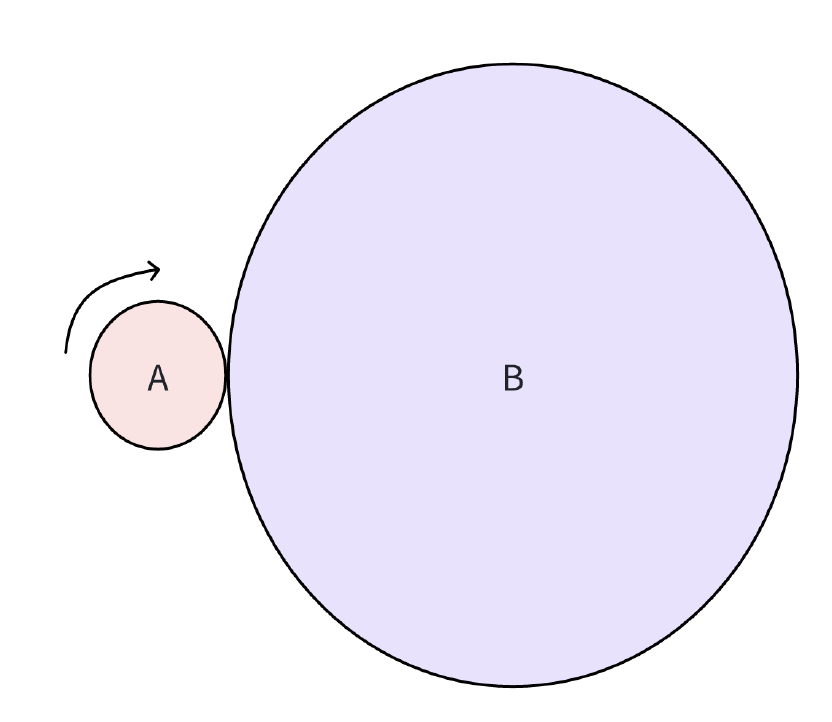
\includegraphics[width=0.8\linewidth]{Figure1.png} 
        \caption{小圆A绕大圆B滚动}
        \label{fig:fig1}
    \end{minipage}\hfill
    \begin{minipage}{0.45\textwidth}
        \centering
        % The user needs to provide the image file 'figure2.png'
        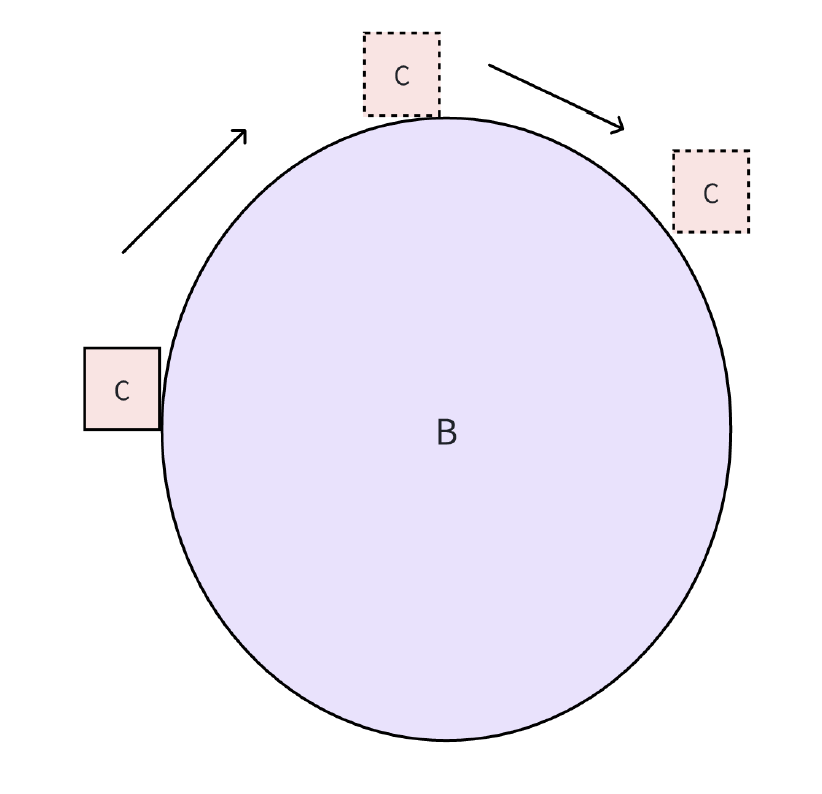
\includegraphics[width=0.8\linewidth]{Figure2.png}
        \caption{正方形C沿大圆B移动}
        \label{fig:fig2}
    \end{minipage}
\end{figure}


\subsection*{3. 正态分布}
概率论和微积分是一个quant需要熟练掌握的基础知识, 小U正在温习正态分布的相关内容。设 $\varphi(y)$ 和 $\Phi(y)$ 分别为标准正态分布的密度和分布函数, 求:

$$\int_{-\infty}^{+\infty}{\left(y+\frac{1}{\sqrt{\pi}}\right)^{2}(1-\Phi(y))\varphi
  (y)dy}$$
令要求解的积分为I,我们将采用对称性和分部积分法来解决。:
$$ I = \int_{-\infty}^{+\infty}{\left(y+\frac{1}{\sqrt{\pi}}\right)^{2}(1-\Phi(y))\varphi(y)dy} $$

\subsection*{1. 对称性换元}
我们利用标准正态分布的两个关键性质:密度函数 $\varphi(y)$ 是一个偶函数以及分布函数满足 $\Phi(-y) = 1 - \Phi(y)$

在积分 $I$ 中,令 $z = -y$,则 $y = -z$ ,得到:
$$ I = \int_{-\infty}^{+\infty}{\left(z-\frac{1}{\sqrt{\pi}}\right)^{2}(1-(1-\Phi(z)))\varphi(z)dz} $$
将变量 $z$ 换回 $y$,我们得到一个与原式等价的积分表达式:
$$ I = \int_{-\infty}^{+\infty}{\left(y-\frac{1}{\sqrt{\pi}}\right)^{2}\Phi(y)\varphi(y)dy} $$

\subsection*{2. 求解}
将两个等价的 $I$ 表达式相加,得到 $2I$:
$$ 2I = \int_{-\infty}^{+\infty} \left[ \left(y+\frac{1}{\sqrt{\pi}}\right)^{2}(1-\Phi(y)) + \left(y-\frac{1}{\sqrt{\pi}}\right)^{2}\Phi(y) \right] \varphi(y)dy $$
化简表达式得到:
$$ 2I = \int_{-\infty}^{+\infty} \left[ y^2 + \frac{1}{\pi} + \frac{2y}{\sqrt{\pi}}(1-2\Phi(y)) \right] \varphi(y)dy $$
现在,我们将积分拆分为三个部分:
$$ 2I = \int_{-\infty}^{+\infty} y^2 \varphi(y)dy + \frac{1}{\pi}\int_{-\infty}^{+\infty}\varphi(y)dy + \frac{2}{\sqrt{\pi}}\int_{-\infty}^{+\infty} y(1-2\Phi(y))\varphi(y)dy $$

\subsection*{3. 计算各部分积分}
\begin{itemize}
    \item \textbf{第一部分}: $\int_{-\infty}^{+\infty} y^2 \varphi(y)dy$ 是标准正态分布的二阶矩,等于其方差,即 \textbf{1}。
    \item \textbf{第二部分}: $\frac{1}{\pi}\int_{-\infty}^{+\infty}\varphi(y)dy$。根据概率密度函数的定义,$\int_{-\infty}^{+\infty}\varphi(y)dy=1$。所以,该项等于 \textbf{$\frac{1}{\pi}$}。
    \item \textbf{第三部分}: $\frac{2}{\sqrt{\pi}} \left[ \int y\varphi(y)dy - 2\int y\Phi(y)\varphi(y)dy \right]$
        \begin{itemize}
            \item 其中 $\int_{-\infty}^{+\infty} y\varphi(y)dy$ 是标准正态分布的均值,等于 0。
            \item 对于 $\int_{-\infty}^{+\infty} y\Phi(y)\varphi(y)dy$,通过分部积分可得其值为 $\frac{1}{2\sqrt{\pi}}$,具体计算过程见附录。
    
            \item 因此,第三部分的值为:$\frac{2}{\sqrt{\pi}} \left[ 0 - 2 \left( \frac{1}{2\sqrt{\pi}} \right) \right] = -\frac{2}{\pi}$。
        \end{itemize}
\end{itemize}

\subsection*{4. 汇总结果}
将三部分的结果代入 $2I$ 的表达式:
$$ 2I = 1 + \frac{1}{\pi} - \frac{2}{\pi} = 1 - \frac{1}{\pi} $$
最终,求解 $I$:
$$ I = \frac{1}{2} - \frac{1}{2\pi} $$

\subsection*{4. 打家劫舍}
小U在复习完数学后觉得coding也不能落下, 请聪明的你帮他设计一个时间复杂度尽可能小的算法, 求一个整数数组S中不含相邻元素的子序列的最大和。

我们考虑动态规划的方法来解决当前问题,可以取得理论最优的时间复杂度O(n)和空间复杂度O(1)。具体来说,我们从第一数组元素遍历每一个元素,
每一次比较获取之前的元素和获取当前元素的数组和哪一个更大。
\begin{lstlisting}[language=Python, caption=O(1) 空间复杂度 和 O(n) 时间复杂度的解法]
    def rob_optimized(S):
        """
        计算不含相邻元素的子序列的最大和
        param S: 一个整数数组
        return: 不含相邻元素的子序列的最大和
        """
        n = len(S)
        if n == 0:
            return 0
        
        # prev_max: 相当于 dp[i-2]
        # curr_max: 相当于 dp[i-1]
        prev_max = 0
        curr_max = 0
    
        for amount in S:
            # temp 用来临时存储 curr_max (即旧的 dp[i-1])
            temp = curr_max
            # 新的 curr_max (即 dp[i]) 是获取前一个元素的最大值(curr_max)与获得当前元素(amount + prev_max)的较大值
            curr_max = max(curr_max, amount + prev_max)
            # 更新 prev_max 为旧的 curr_max,为下一次迭代做准备
            prev_max = temp
    
        return curr_max
    # --- 示例数组 ---
    example_S = [2, 7, 9, 3, 1]

    # --- 调用函数并打印结果 ---
    max_sum = rob_optimized(example_S)
    print(f"对于示例数组 S = {example_S}")
    # 对于示例数组 S = [2, 7, 9, 3, 1]
    print(f"不含相邻元素的最大和为: {max_sum}") 
    # 不含相邻元素的最大和为: 12
\end{lstlisting}

\subsection*{5. Linear Regression Model}
Xiao U is learning English and regression analysis. Please help him solve the following problem:
Suppose we have a simple linear regression model,
$$ y_{j}=\beta_{0}+\beta_{1}x_{j}+\epsilon_{j}, \quad j=1,2,...,n $$
But the $x_{j}$ are independently $N(\mu_{x},\sigma_{x}^{2})$. We assume further that $\epsilon_{j}\sim N(0,\sigma_{e}^{2})$, independently of the $x_{j}$'s.
Suppose further that $x_{j}$ is in fact measured with error, so the observations are $(y_{j},w_{j})$, where
$$ w_{j}=x_{j}+u_{j}, \quad u_{j}\sim N(0,\sigma_{u}^{2}) $$
and $u$ is independent of both $x$ and $\epsilon$.
Now, please show that $E(y_{j}|w_{j})=\alpha_{0}+\alpha_{1}w_{j}$, and give expressions for $\alpha_{0}$ and $\alpha_{1}$ as functions of known constants.

因为$E(y_{j}|w_{j})=E(\beta_{0}+\beta_{1}x_{j}+\epsilon_{j}|w_{j})=\beta_{0}+E(\beta_{1}x_{j}+\epsilon_{j}|w_{j})=\beta_{0}+\beta_{1}E(x_{j}|w_{j})+E(\epsilon_{j}|w_{j})$
又因为$\epsilon_{j}$与$w_{j}$独立,所以$E(\epsilon_{j}|w_{j})=E(\epsilon_{j})=0$

对于$E(x_{j}|w_{j})$,我们可以应用附录中证明的正态分布条件期望公式。在本题中,$x_j$和$w_j$构成二元正态随机变量,其中:
\begin{itemize}
    \item $E(x_j) = \mu_x$
    \item $Var(x_j) = \sigma_x^2$
    \item $E(w_j) = E(x_j + u_j) = \mu_x + 0 = \mu_x$
    \item $Var(w_j) = Var(x_j + u_j) = \sigma_x^2 + \sigma_u^2$
    \item $Cov(x_j, w_j) = Cov(x_j, x_j + u_j) = Cov(x_j, x_j) + Cov(x_j, u_j) = \sigma_x^2 + 0 = \sigma_x^2$
\end{itemize}

根据附录中的条件期望公式:
$$E(X|Y=y) = E(X) + \frac{Cov(X,Y)}{Var(Y)}(y - E(Y))$$

代入我们的参数:
$$
E(x_{j}|w_{j}) = \mu_{x} + \frac{\sigma_{x}^{2}}{\sigma_{x}^{2} + \sigma_{u}^{2}}(w_{j} - \mu_{x})
$$
因此:
$$E(y_{j}|w_{j}) = \beta_{0} + \beta_{1}\left[\mu_{x} + \frac{\sigma_{x}^{2}}{\sigma_{x}^{2} + \sigma_{u}^{2}}(w_{j} - \mu_{x})\right]$$

整理得到:
$$E(y_{j}|w_{j}) = \beta_{0} + \beta_{1}\mu_{x}\left(1-\frac{\sigma_{x}^{2}}{\sigma_{x}^{2} + \sigma_{u}^{2}}\right) + \beta_{1}\frac{\sigma_{x}^{2}}{\sigma_{x}^{2} + \sigma_{u}^{2}}w_{j}$$

令$\alpha_{0} = \beta_{0} + \beta_{1}\mu_{x}\left(1-\frac{\sigma_{x}^{2}}{\sigma_{x}^{2} + \sigma_{u}^{2}}\right)$,$\alpha_{1} = \beta_{1}\frac{\sigma_{x}^{2}}{\sigma_{x}^{2} + \sigma_{u}^{2}}$

则:
$$E(y_{j}|w_{j}) = \alpha_{0} + \alpha_{1}w_{j}$$
\subsection*{6. 共半球问题}
\subsubsection*{(1)}
小U发现了一道经典的量化题: 圆上随机取N个点, 它们在同一个半圆内的概率有多大?

让我们先任意选择一个点,比如 \(P_1\),以 $P_1$ 为起点,顺时针画出一个半圆。我们称这个半圆为 $H_1$。要让所有其他 $N-1$ 个点都落在这个特定的半圆 $H_1$ 内,概率是多少?
\begin{itemize}
    \item 对于任何一个随机点 $P_i$ ($i \neq 1$),它落在 $H_1$ 内的概率是 $\frac{1}{2}$。
    \item 因为这 $N-1$ 个点的选择是相互独立的,所以它们全部落在 $H_1$ 内的概率是 $(\frac{1}{2})^{N-1}$。
\end{itemize}
并计这个事件为事件$A_i$,
\begin{itemize}
    \item $A_1$: 所有点都落在以 $P_1$ 为起点的顺时针半圆内。
    \item $A_2$: 所有点都落在以 $P_2$ 为起点的顺时针半圆内。
    \item \dots
    \item $A_N$: 所有点都落在以 $P_N$ 为起点的顺时针半圆内。
\end{itemize}
注意到,这N个事件的互斥的,且根据对称性,其概率相同均为$(\frac{1}{2})^{N-1}$。
\subsubsection*{(2)}
求知欲很强的小U继续探索, 假如问题变成3维球体呢? 即在球面上随机取N个点, 它们在同一个半球内的概率有多大?

事件是“所有N个点都落在某一个半球内”,同样,我们先任意选择一个点 $P_1$。这个点 $P_1$ 可以被看作是某个半球的“极点”。这个半球 $H_1$ 就是由过球心且垂直于 $\vec{OP_1}$ 向量的平面所定义的、$P_1$ 所在的那一半球面。
要让所有其他 $N-1$ 个点都落在这个特定的半球 $H_1$ 内,概率为$(\frac{1}{2})^{N-1}$。我们同样定义 $N$ 个事件 $A_i$:所有其他 $N-1$ 个点都落在以 $P_i$ 为“极点”的那个半球内。正如在二维情况中一样,这些事件也是相互排斥的。
$$ P(\text{所有点在同一个半球内}) = \sum_{i=1}^{N} P(A_i) = N \times \left(\frac{1}{2}\right)^{N-1} $$
\subsubsection*{(3) 【拓展思考题】}
在n维空间的球面上随机取N个点, 它们在同一个半球内的概率有多大?

类似的,维度的增加并没有改变问题的实质。在 $n$ 维空间中,一个“超半球”(hyper-hemisphere)是由一个通过球心的 $(n-1)$ 维超平面(hyperplane)将 $(n-1)$-球面切割成两半而得到的。
。因此,一个随机点落在指定超半球内的概率永远是 $\frac{1}{2}$。类似的事件$A_i$也是相互排斥的,且根据对称性,其概率相同均为$(\frac{1}{2})^{N-1}$。
$$ P(\text{所有点在同一个超半球内}) = \sum_{i=1}^{N} P(A_i) = N \times \left(\frac{1}{2}\right)^{N-1} $$
\subsection*{7. Pattern Problem}
小U在学习stochastic process, 他手里有一个不均匀的硬币, 每次掷到正面(H)的概率为p, 掷到反面(T)的概率为q, $p+q=1$, 请问首次掷到以下pattern的期望投掷次数为多少?
\begin{enumerate}
    \item HHHHHHTTTTTT
    \item HHHHHHHHHHHH
    \item HTHTHTTHTHT
\end{enumerate}



\section*{附录}

\subsection*{正态分布概率密度函数推导}
首先我们先证明正态分布概率密度函数有如下性质:
$$
\begin{align*}
    \varphi'(y) &= \frac{d}{dy}\left(\frac{1}{\sqrt{2\pi}}e^{-\frac{y^2}{2}}\right) \\
    &= \frac{1}{\sqrt{2\pi}} \cdot \frac{d}{dy}\left(e^{-\frac{y^2}{2}}\right) \\
    &= \frac{1}{\sqrt{2\pi}} \cdot e^{-\frac{y^2}{2}} \cdot \left(-y\right) \\
    &= -y \cdot \frac{1}{\sqrt{2\pi}}e^{-\frac{y^2}{2}} \\
    &= -y \cdot \varphi(y)
\end{align*}
$$
接着我们可以推导出:
$$
\begin{align*}
    \int_{-\infty}^{+\infty} y\Phi(y)\varphi(y)dy
    &= -\int_{-\infty}^{+\infty} \Phi(y)d(-\varphi(y)) \\
    &= -\left[\Phi(y)(-\varphi(y))\right]_{-\infty}^{+\infty} + \int_{-\infty}^{+\infty} \varphi(y)d\Phi(y) \\
    &= -\left[\Phi(y)(-\varphi(y))\right]_{-\infty}^{+\infty} + \int_{-\infty}^{+\infty} \varphi(y)^2 dy \\
    &= 0 + \int_{-\infty}^{+\infty} \frac{1}{2\pi}e^{-y^2} dy \\
    &= \frac{1}{2\pi} \cdot \sqrt{\pi} \\
    &= \frac{1}{2\sqrt{\pi}}
\end{align*}
$$

\subsection*{证明正态分布的条件期望公式}
\noindent 证明过程的核心思想是:
\begin{enumerate}
    \item 写出 X 和 Y 的联合概率密度函数 $f(x, y)$。
    \item 写出 Y 的边缘概率密度函数 $f_Y(y)$。
    \item 利用公式 $f_{X|Y}(x|y) = \frac{f(x, y)}{f_Y(y)}$ 求出在 Y=y 的条件下 X 的条件概率密度函数。
    \item 这个条件概率密度函数本身也是一个正态分布,它的期望值就是我们要求的 $E(X|Y=y)$。
\end{enumerate}

\hrule
\vspace{1em}

\subsection*{第一步:定义联合概率密度函数 }

设随机变量 $(X, Y)$ 服从双变量正态分布,其参数如下:
\begin{itemize}
    \item 均值:$E(X) = \mu_X$, $E(Y) = \mu_Y$
    \item 方差:$Var(X) = \sigma_X^2$, $Var(Y) = \sigma_Y^2$
    \item 相关系数:$Corr(X, Y) = \rho$
\end{itemize}

其联合概率密度函数 $f(x, y)$ 的核心在于指数部分。我们可以将指数部分记为 $-\frac{1}{2}Q(x,y)$,其中:
$$
Q(x,y) = \frac{1}{1-\rho^2} \left[ \left(\frac{x-\mu_X}{\sigma_X}\right)^2 - 2\rho\left(\frac{x-\mu_X}{\sigma_X}\right)\left(\frac{y-\mu_Y}{\sigma_Y}\right) + \left(\frac{y-\mu_Y}{\sigma_Y}\right)^2 \right]
$$

\subsection*{第二步:分解指数项}

在这里,我们把所有和 $x$ 相关的项整理成一个平方项。$Q(x, y)$ 中和 $x$ 相关的部分可以看作是关于变量 $(\frac{x-\mu_X}{\sigma_X})$ 的二次方程。我们把它配成一个完全平方:
\begin{align*}
Q(x,y) &= \frac{1}{1-\rho^2} \left\{ \left[ \left(\frac{x-\mu_X}{\sigma_X}\right) - \rho\left(\frac{y-\mu_Y}{\sigma_Y}\right) \right]^2 + (1-\rho^2)\left(\frac{y-\mu_Y}{\sigma_Y}\right)^2 \right\} \\
&= \frac{1}{1-\rho^2} \left[ \left(\frac{x-\mu_X}{\sigma_X}\right) - \rho\left(\frac{y-\mu_Y}{\sigma_Y}\right) \right]^2 + \left(\frac{y-\mu_Y}{\sigma_Y}\right)^2
\end{align*}
这个形式非常重要,因为它成功地将表达式分离成两部分:一个同时包含 $x$ 和 $y$ 的平方项,以及一个只包含 $y$ 的项。

\subsection*{第三步:导出条件概率密度函数}

现在我们可以重写整个联合概率密度函数 $f(x,y)$。代入我们分解后的 $Q(x,y)$,并利用指数性质 $e^{A+B} = e^A e^B$,我们可以把表达式拆开:
\begin{align*}
f(x,y) &= \frac{1}{2\pi\sigma_X\sigma_Y\sqrt{1-\rho^2}} \exp\left(-\frac{1}{2}Q(x,y)\right) \\
&= \underbrace{\left[ \frac{1}{\sqrt{2\pi}\sigma_Y} \exp\left( -\frac{(y-\mu_Y)^2}{2\sigma_Y^2} \right) \right]}_{f_Y(y)} \\
& \quad \times \underbrace{\left[ \frac{1}{\sqrt{2\pi}\sigma_X\sqrt{1-\rho^2}} \exp\left( -\frac{\left[ \left(\frac{x-\mu_X}{\sigma_X}\right) - \rho\left(\frac{y-\mu_Y}{\sigma_Y}\right) \right]^2}{2(1-\rho^2)} \right) \right]}_{f_{X|Y}(x|y)}
\end{align*}
根据条件概率的定义 $f(x,y) = f_Y(y) \cdot f_{X|Y}(x|y)$,我们成功地将联合PDF分解为了边缘PDF和条件PDF的乘积。

\subsection*{第四步:条件分布的期望}

现在我们仔细观察条件概率密度函数 $f_{X|Y}(x|y)$。我们可以把它整理成一个标准正态分布PDF的形式 $\frac{1}{\sqrt{2\pi}\sigma_{\text{new}}}\exp(-\frac{(x-\mu_{\text{new}})^2}{2\sigma_{\text{new}}^2})$。
$$
f_{X|Y}(x|y) = \frac{1}{\sqrt{2\pi}\sigma_X\sqrt{1-\rho^2}} \exp\left( -\frac{\left( x - \left[ \mu_X + \rho\frac{\sigma_X}{\sigma_Y}(y-\mu_Y) \right] \right)^2}{2\sigma_X^2(1-\rho^2)} \right)
$$
通过与标准形式对比,我们可以直接读出这个条件分布的期望(均值)和方差:
\begin{itemize}
    \item \textbf{条件期望 (均值):} $\mu_{\text{new}} = E(X|Y=y) = \mu_X + \rho\frac{\sigma_X}{\sigma_Y}(y-\mu_Y)$
    \item \textbf{条件方差:} $\sigma_{\text{new}}^2 = Var(X|Y=y) = \sigma_X^2(1-\rho^2)$
\end{itemize}

\subsection*{第五步:代入协方差}

我们已经得到了条件期望的表达式,现在只需将其转换成用协方差表示的形式。根据定义,相关系数 $\rho = \frac{Cov(X,Y)}{\sigma_X\sigma_Y}$。将其代入我们得到的期望公式中:
\begin{align*}
E(X|Y=y) &= \mu_X + \left( \frac{Cov(X,Y)}{\sigma_X\sigma_Y} \right) \frac{\sigma_X}{\sigma_Y} (y-\mu_Y) \\
&= \mu_X + \frac{Cov(X,Y)}{\sigma_Y^2} (y-\mu_Y)
\end{align*}
最后,将 $\mu_X$, $\mu_Y$, $\sigma_Y^2$ 替换为期望和方差的符号即可:
$$
E(X|Y=y) = E(X) + \frac{Cov(X,Y)}{Var(Y)}(y - E(Y))
$$
从而完成证明。

\end{document}